\section{Discussion}\label{sec:discussion}

\subsection{Learning}\label{subsec:learning}

Using real world brain scans of a very low resolution, we've been able to achieve excellent classification using both
2 dimensional and 3 dimensional convolutional networks, with somewhat promising generalizability to previously unseen subjects.
The models have been very able to differentiate when a subject was scanned viewing a tempting food image against when the image
presented is neutral, where I personally can see absolutely no clear difference.

Unsurprisingly deeper architectures also tend to improve performance marginally,
as they can cope with increasingly subtle changes presumably, in both the performance of the 2d and 3d CNN's

While we may have empirically found improved performance using 3 dimensional CNN's over all alternatives,
the hefty cost of computation has proven difficult to cope with and limited the ability to explore segmentation farther.

\subsection{Future Works}\label{subsec:future-works}

While classification feels well proven and a desirable performance was achieved,
the natural next step is to try an highlight what the network has learned to recognize
as indicative of a particular stimuli, turning the blackbox computation into a powerful teacher.
My attempts made to the point of this submission to adapt the classifiers to unsupervised segmentation
have not yet been fully successful.

\subsubsection{Refinements}\label{refinements}

Refinements to the classifier are always a worthwhile endeavor, though this particular classification feels well
handled by the chosen architectures at relatively shallow levels.

Given the promise of warm-starts progressing learning, I'd be very interested in exploring different
learning rate schedulers to see what combination of minute and aggressive changes lands the model in the most performant
optimization.

Lastly as there's typically a free boost from using an ensemble model, I'd be interested in exploring what combination
of models yields a more robust cohesive model which generalizes very well to previously unseen subject's brain scans.

\subsubsection{Visualizations}\label{fw-viz}

The models are also naturally capable of producing visualizations of their convolutional filters, class representations
and creating saliency maps.

In figure~\ref{fig:saliency} we see one example of Saliency maps in action.
Interestingly enough the model does not key strongly off of discrete brain structures as I had assumed it would.
I speculate that the data being so downgraded provides difficulty in precisely conveying brain activity and the models
are instead forced to learn off of other subtle activities across the brain, which are of course not fully silent during
the passive image viewing task.

 \begin{figure}
  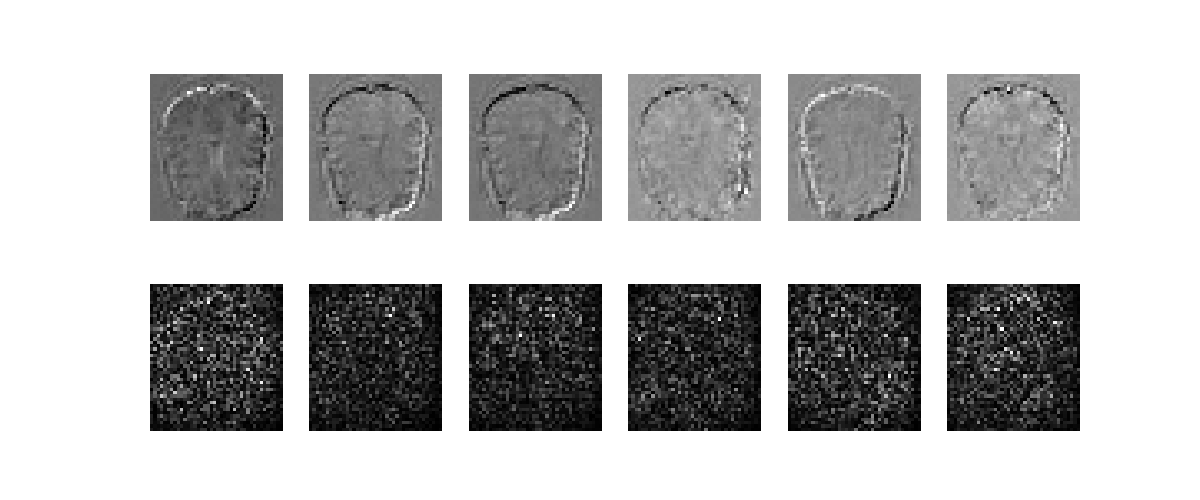
\includegraphics[width=\linewidth]{images/saliency.png}
  \caption{Three Nonfood \& Three Food Brain Scan Slices with their respective Saliency Maps}
  \label{fig:saliency}
\end{figure}



